\lhead{\emph{Results}} 
\chapter{Results}

The experiment was performed 16 times with 6 different people. The
results were analyzed taken into account the previous descripted metrics
and from different perspectives that are reflected in the following 5
plots that are commented individually.

\begin{figure}[!ht]
\centering
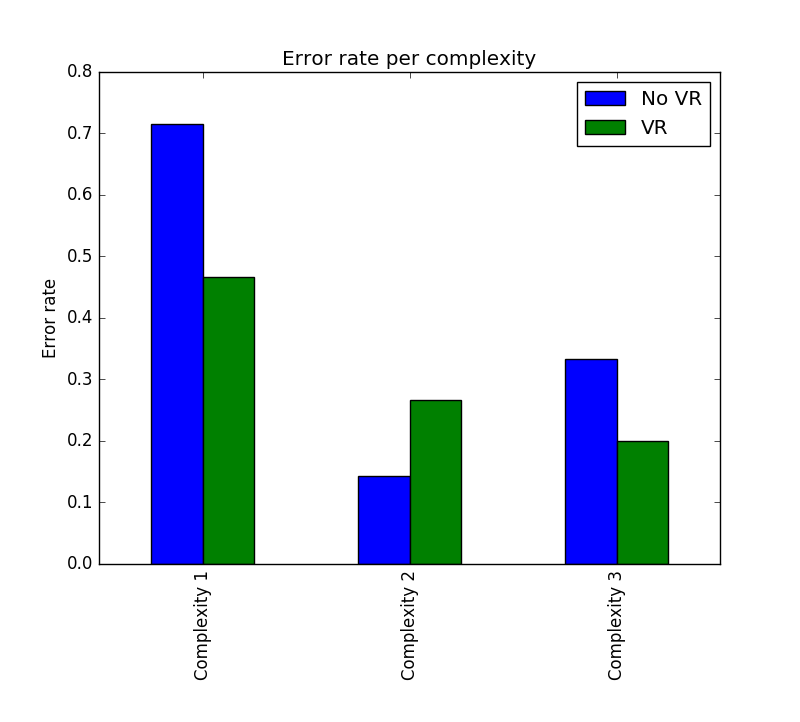
\includegraphics[scale=0.33]{image1.png}
\caption{Error rate per complexity level and condition} \label{fig:plot1}
\end{figure}

Figure \ref{fig:plot1} shows how the X axis is split up in three complexity
levels and the Y axis measures the average error rate in each complexity
level. The first interesting thing that can be observed in this plot is
that in the first and third complexity levels, the error rate produced
with no use of VR is higher than the error rate when the subjects used
VR to visualize the graph. This was expected because the use of VR
should make easier the task of visualizing graphs. However, in the
second complexity level happens exactly the opposite. This fact was
completely unexpected and it's difficult to make a conclusion about this
distortion.

If we take the mean of the percentage of correct answers, that is the
inverse of the error rate, the percentage that corresponds to the use of
VR is 68.89\%. This is slightly higher than the percentage of correct
answers without the use of VR, that is 60.47\%. This is not a big
difference in performance, but follows the tendency proposed in the
paper.

\protect\hypertarget{transcription-of-the-thomas-talk-last-pr}{}{}On the
other hand, independently if we use VR or not, the error rate in the
first complexity level is rather higher than the other two complexity
levels. This means the opposite of what we expected and what we found in
the original paper. That's it, the error rate should increase
proportionally to the level of complexity. The explanation we give for
this is that the subjects that visualize the graphs for the first time
must get used to the device and the experiment, and this learning
process takes some time that we didn't provide. Therefore, we could say
that this was an issue caused by the lack of familiarity with the device
and the experiment.

\begin{figure}[!ht]
\centering
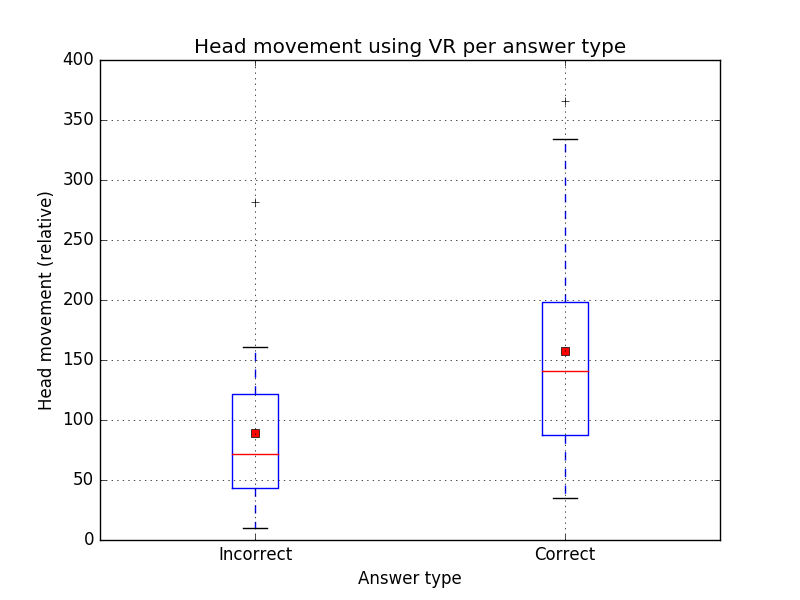
\includegraphics[scale=0.33]{image2.png}
\caption{Head movement using VR per answer type} \label{fig:plot2}
\end{figure}

In figure \ref{fig:plot2} , we can see the amount of head movement produced every time
a subject provided either an incorrect or a correct answer. This
relation wasn't discussed in the original paper and it provided some
interesting results. The main result was that the amount of head
movement increased a 30.19\% for correct answer with respect to
incorrect answer. That's it, people that moves their head more to
visualize the graph are more likely to do a correct answer. The head
movement was measured using the movement of the camera in the virtual
space in Unity units. It doesn't provide a reference to see how is the
real distance traversed by the head in meters, but it allows us to
compare among different scenarios.

\begin{figure}[!ht]
\centering
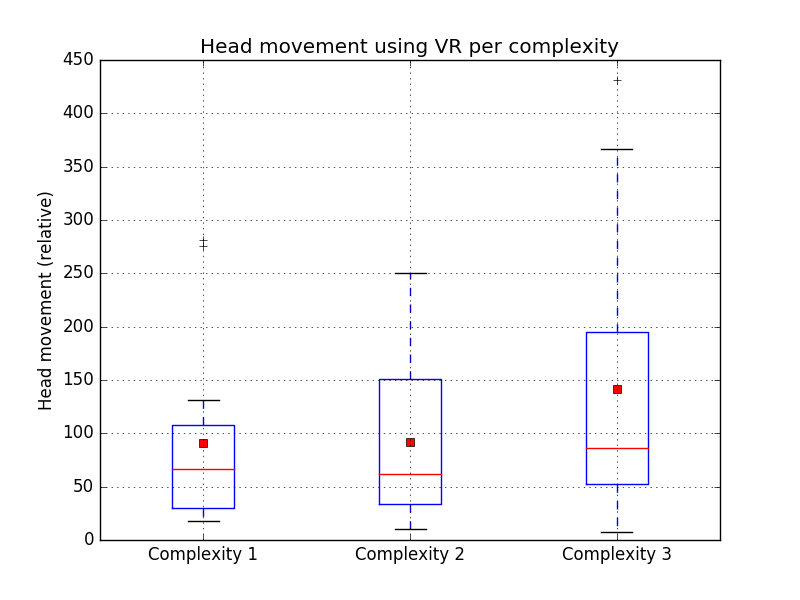
\includegraphics[scale=0.33]{image3.png}
\caption{Head movement using VR per complexity level} \label{fig:plot3}
\end{figure}

Similarly to the previous plot, in figure \ref{fig:plot3}  we can observe again the head movement in the
Y axis and the X axis is split up in three complexity levels. Specially
for the third complexity level, the mean amount of head movement is
slightly higher than the others. This was expected because the
experiment was set up such that people in higher complexity levels have
a higher maximum amount of time and thus, they tend to expend more time
and it results in a higher amount of head movement in total. It can be
seen also that the variance is very high in the third complexity level
due presumably to the fact that people really liked the sensation at
this point of the experiment and they moved their heads to take
advantage of the experience.

\begin{figure}[!ht]
\centering
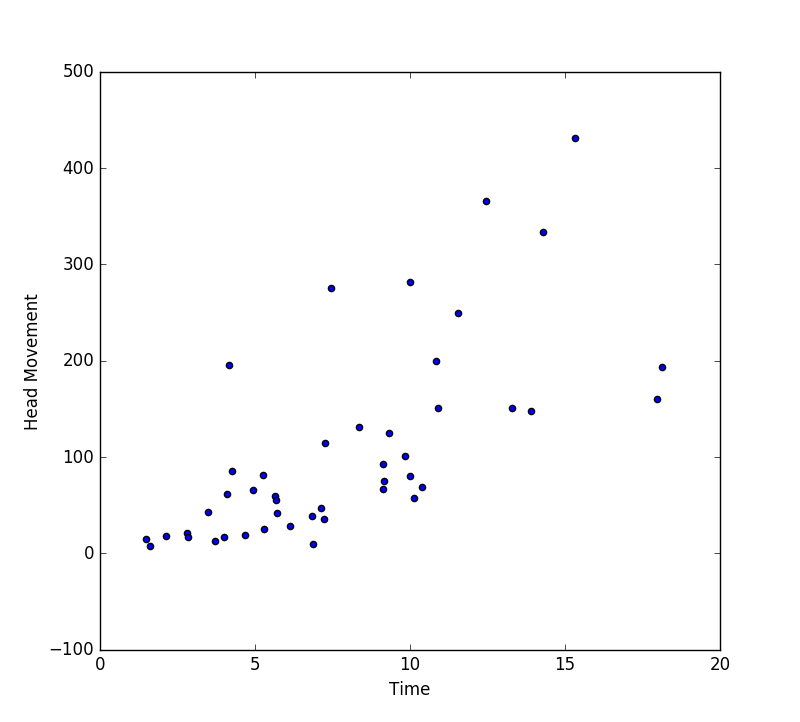
\includegraphics[scale=0.33]{image5.png}
\caption{Head movement and response time (in seconds)} \label{fig:plot5}
\end{figure}

In the scatter plot of figure \ref{fig:plot5} we can observe the same pattern of the previous
plot. Almost all the points are clustered in a range among 0 and 10
seconds and almost all of them has an upper bound of 100 units of head
movements. From this point, the variance starts to grow exponentially as
the number of time increases. This reaffirm the conclusion that when
people have more time to give an answer, they try to see the graph from
a different perspective to be sure that they are providing a correct
answer. Therefore. in scenarios where time is not a constraint to
visualize the graph, people uses more head tracking to comprehend better
the graph.

\begin{figure}[!ht]
\centering
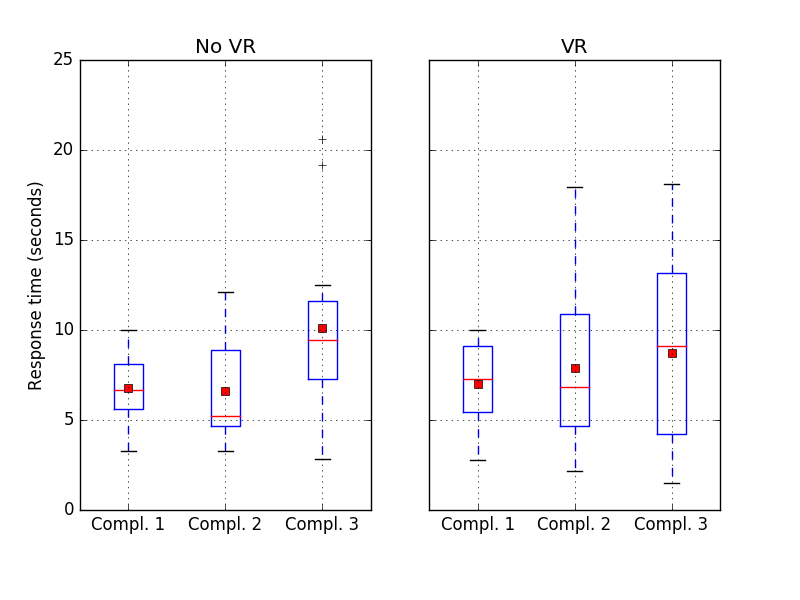
\includegraphics[scale=0.33]{image4.png}
\caption{Response time per complexity level} \label{fig:plot4}
\end{figure}

In the two box plots that are drawn in figure \ref{fig:plot4}, we can see the response time in seconds in the Y
axis, separated firstly in VR and no VR and secondly in the three
complexity levels. We can see for both plots that the higher the graph
complexity is, the is higher is the time a subject takes to answer. This
was of course expected because as the maximum time to answer increases,
people feel less pressure to make a decision. Therefore, we can't be
sure if the graph is really comprehended better or it's just a matter of
it depends on the maximum amount of time provided to answer. This should
be compared with another version of the experiment in which the
information about the maximum amount of time is not provided and see the
real evolution.

We can also see that the variance in the response time is very high
again when VR is used. Again, we think that this is caused because
people really liked the VR experience and some of them spent higher
amounts of time. However, if we observe the means and we compare them,
we can observe they are both practically the same in VR (7.81 seconds)
and No VR (7.88 seconds). Comparing to the paper, this is not what we
expected as the response time should be rather lower when VR is used.

In all the plots we have analyzed, we can observer a common problem: The
sample size is too low to make significant conclusions. Several
technical problems and constraints in the availability of the device led
us to a partial failure in the data collecting. Some of the conclusions
we have made follows the tendency of the ones made in the provided
paper, but we can't give our results the same trustworthiness that the
one in the paper.

For future work, if this experiment would have repeated, we would change
some of the parameters that influences on the results like giving
information to the user about the maximum amount of time to answer. In
addition, we would try to collect a significant amount of data to get
significant and reliable results and compare them with the paper at the
same level of trustworthiness.



